\section{Proposed Method} 

%% TODO: Adjust the size of the figure by using [scale=x] or [widht=.x\linewidth] (x is a fraction) to fit within the frame. Then rename to your picture file name and add the caption
\begin{frame}{Overview}
	\begin{figure}
		\centering
		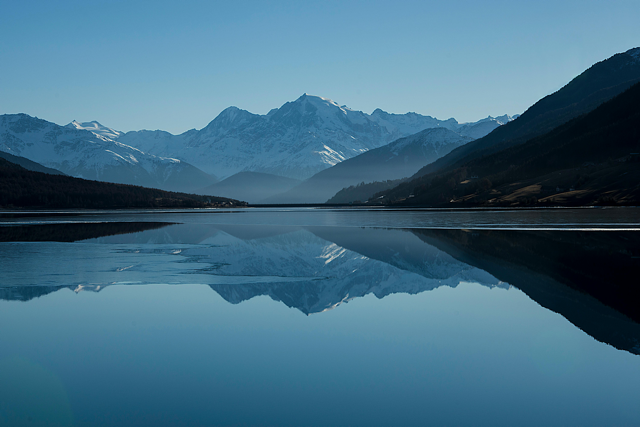
\includegraphics[width=.8\linewidth]{samplel.png}
		\caption{The caption of the figure.}
	\end{figure}	
	%% TODO: You can add the note here
	\note{}
\end{frame}

%% TODO: Uncomment the next four lines to enable this frame
% \begin{frame}{Methodology}
% 	%% TODO: You can add the note here
% 	\note{}
% \end{frame}

\begin{frame}[label=process1]{\texttt{Sample} Process 
  \hyperlink{algo1}{\beamerbutton{Algorithm}} 
  \hyperlink{pseudocode1}{\beamerbutton{Pseudocode}}
}
	\begin{columns}
		\column{0.3\textwidth}
		\centering
		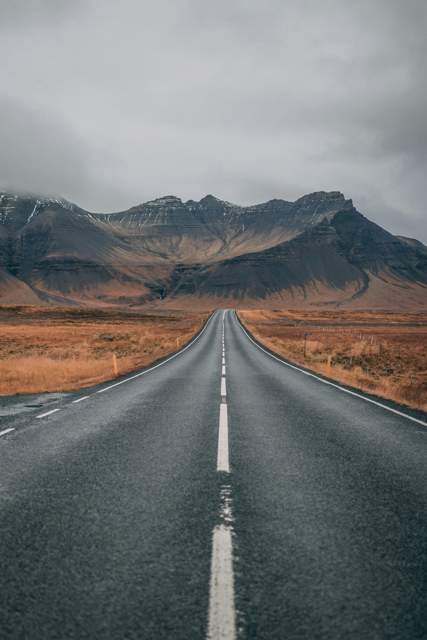
\includegraphics[height=1.8\textwidth]{samplev.png}
		\column{0.7\textwidth}
		\begin{itemize}
			\item \textbf{Goal:}
			\item \textbf{Result:}
			\item \textbf{Step:} 
			\item \textbf{Scope:}
		\end{itemize}
	\end{columns}
	%% TODO: You can add the note here
	\note{}
\end{frame}